\documentclass[border=2pt]{standalone}
\usepackage{fontspec}
\usepackage{unicode-math}
\setmainfont{Libertinus Serif}
\setsansfont{Libertinus Sans}
\setmathfont{Libertinus Math}[Scale=MatchUppercase]
\setmonofont{JetBrainsMono-Regular.ttf}[Path=../fonts/,ItalicFont=JetBrainsMono-Italic.ttf,Scale=0.95,RawFeature={-liga,-calt,-clig,-dlig}]
\usepackage{amsmath}
\providecommand{\llbracket}{[\![}
\providecommand{\rrbracket}{]\!]}
\usepackage{tikz}
\usetikzlibrary{positioning,arrows.meta,fit,backgrounds,calc,decorations.pathreplacing,decorations.markings,shapes.misc,matrix,shadings}

\definecolor{ink}{HTML}{1F2328}
\definecolor{muted}{HTML}{5B6470}
\definecolor{hairline}{HTML}{C9CFD6}
\definecolor{paper}{HTML}{FFFFFF}
\definecolor{pass}{HTML}{007A59}   \definecolor{passsoft}{HTML}{DAF1E9}
\definecolor{back}{HTML}{7A3E65}   \definecolor{backsoft}{HTML}{F1E1EB}
\definecolor{backdeep}{HTML}{70355C}
\definecolor{keep}{HTML}{006A91}   \definecolor{keepsoft}{HTML}{DCE9F5}
\definecolor{meas}{HTML}{9A5B00}   \definecolor{meassoft}{HTML}{FBEFD5}
\definecolor{measdeep}{HTML}{885000}
\definecolor{bad}{HTML}{AF4900}    \definecolor{badsoft}{HTML}{F9E1D3}
\definecolor{light}{HTML}{167BB4}  \definecolor{lightsoft}{HTML}{E3F2FB}

\tikzset{
  house/.style={>={Stealth[length=1.35mm, width=.95mm]}, line width=0.6pt,
    every node/.style={font=\small, text=ink}},
  flowmark/.style={postaction={decorate},decoration={markings,
    mark=at position .60 with {\arrow{Stealth[length=1.15mm,width=.8mm]}}}},
  box/.style={draw=ink, line width=0.6pt, rounded corners=1.8pt, inner xsep=5pt, inner ysep=3.5pt,
    align=center, fill=paper},
  boxdim/.style={box, draw=hairline, text=muted},
  boxpass/.style={box, draw=pass, shade,left color=passsoft!45!white,right color=passsoft},
  boxback/.style={box, draw=back, shade,left color=backsoft!45!white,right color=backsoft},
  boxkeep/.style={box, draw=keep, shade,left color=keepsoft!45!white,right color=keepsoft},
  boxmeas/.style={box, draw=meas, shade,left color=meassoft!45!white,right color=meassoft},
  boxbad/.style={box, draw=bad, shade,left color=badsoft!45!white,right color=badsoft},
  body/.style={box, shade,top color=white,bottom color=ink!5!white,
    minimum width=10mm, minimum height=11mm, font=\normalsize},
  wire/.style={draw=ink, line width=0.8pt},
  wpass/.style={draw=pass, line width=0.9pt},
  wback/.style={draw=back, line width=0.9pt},
  wkeep/.style={draw=keep, line width=0.9pt},
  wmeas/.style={draw=meas, line width=0.9pt},
  cwire/.style={draw=ink, line width=0.4pt, double, double distance=1.1pt},
  cmeas/.style={draw=meas, line width=0.45pt, double, double distance=1.1pt},
  flow/.style={->, draw=ink, line width=0.6pt},
  flowdim/.style={->, draw=muted, line width=0.5pt},
  lab/.style={font=\footnotesize, text=ink, inner sep=1.5pt},
  labpass/.style={lab, text=pass!80!black},
  labback/.style={lab, text=backdeep},
  labkeep/.style={lab, text=keep},
  labmeas/.style={lab, text=measdeep},
  labbad/.style={lab, text=bad},
  note/.style={font=\footnotesize, text=muted, align=left, inner sep=1.5pt},
  head/.style={font=\small\bfseries, text=ink, inner sep=1.5pt},
  panel/.style={font=\footnotesize\itshape, text=muted, inner sep=1.5pt},
  group/.style={draw=hairline, dashed, rounded corners=2.5pt, inner sep=5pt},
  gate/.style={draw=ink, fill=paper, line width=0.6pt, rounded corners=1.2pt, minimum size=6mm, inner sep=2pt},
  ctrl/.style={circle, fill=ink, inner sep=0pt, minimum size=1.6mm},
  octrl/.style={circle, draw=ink, fill=paper, inner sep=0pt, minimum size=1.6mm, line width=0.6pt},
  dot/.style={circle, fill=ink, inner sep=0pt, minimum size=1.5mm},
  meter/.style={draw=meas, fill=meassoft, line width=0.6pt, rounded corners=1.2pt, minimum width=7mm,
    minimum height=5.6mm, inner sep=0pt,
    path picture={\draw[measdeep, line width=0.5pt] ($(path picture bounding box.center)+(-2mm,-1.2mm)$) arc (180:0:2mm);
                  \draw[measdeep, line width=0.5pt, ->] ($(path picture bounding box.center)+(0,-1.2mm)$) -- ++(1.4mm,2.1mm);}},
  cell/.style={draw=hairline, minimum width=7mm, minimum height=5.5mm, inner sep=0pt, font=\footnotesize},
}
\newcommand{\feedbackcurve}[3]{\draw[wback, postaction={decorate}, decoration={markings, mark=at position .5 with {\arrow{Stealth[length=1.3mm,width=.9mm]}}}]
    ($(#1.east)+(0,-2.6mm)$) -- ($(#1.east)+({max(#3-0.55,0.15)},-2.6mm)$)
    to[out=0,in=0,looseness=1.7] ($(#1.east)+({max(#3-0.55,0.15)},-2.6mm)+(0,-#2)$)
    -- ($(#1.west)+({-max(#3-0.55,0.15)},-2.6mm)+(0,-#2)$)
    to[out=180,in=180,looseness=1.7] ($(#1.west)+({-max(#3-0.55,0.15)},-2.6mm)$)
    -- ($(#1.west)+(0,-2.6mm)$);}
\newcommand{\feedbackcurvez}[4]{\draw[wback]
    ($(#1.east)+(0,-2.6mm)$) -- ($(#1.east)+({max(#3-0.55,0.15)},-2.6mm)$)
    to[out=0,in=0,looseness=1.7] ($(#1.east)+({max(#3-0.55,0.15)},-2.6mm)+(0,-#2)$)
    -- node[boxback, font=\footnotesize, inner xsep=3pt, inner ysep=2pt] {#4}
       ($(#1.west)+({-max(#3-0.55,0.15)},-2.6mm)+(0,-#2)$)
    to[out=180,in=180,looseness=1.7] ($(#1.west)+({-max(#3-0.55,0.15)},-2.6mm)$)
    -- ($(#1.west)+(0,-2.6mm)$);
  \draw[wback,-{Stealth[length=1.3mm,width=.9mm]}] ($(#1.west)+(-0.12,-2.6mm)+(0,-#2)$) -- ++(-0.01,0);}
\newcommand{\feedbackcurveat}[4]{\draw[wback, postaction={decorate}, decoration={markings, mark=at position .5 with {\arrow{Stealth[length=1.3mm,width=.9mm]}}}]
    ($(#1.east)+(0,-#2)$) -- ($(#1.east)+({max(#4-0.55,0.15)},-#2)$)
    to[out=0,in=0,looseness=1.7] ($(#1.east)+({max(#4-0.55,0.15)},-#2)+(0,-#3)$)
    -- ($(#1.west)+({-max(#4-0.55,0.15)},-#2)+(0,-#3)$)
    to[out=180,in=180,looseness=1.7] ($(#1.west)+({-max(#4-0.55,0.15)},-#2)$)
    -- ($(#1.west)+(0,-#2)$);}
\newcommand{\backloop}[3]{\draw[wback, rounded corners=3pt] ($(#1.east)+(0,-2.6mm)$) -- ++(#3,0) -- ++(0,-#2) -- ($(#1.west)+(-#3,-2.6mm)+(0,-#2)$) -- ($(#1.west)+(-#3,-2.6mm)$) -- ($(#1.west)+(0,-2.6mm)$);}
\newcommand{\ket}[1]{\lvert #1\rangle}
\newcommand{\bra}[1]{\langle #1\rvert}
\newcommand{\kw}[1]{\texttt{#1}}
\providecommand{\Tr}{\operatorname{Tr}}
\hyphenpenalty=10000 \exhyphenpenalty=10000

\begin{document}
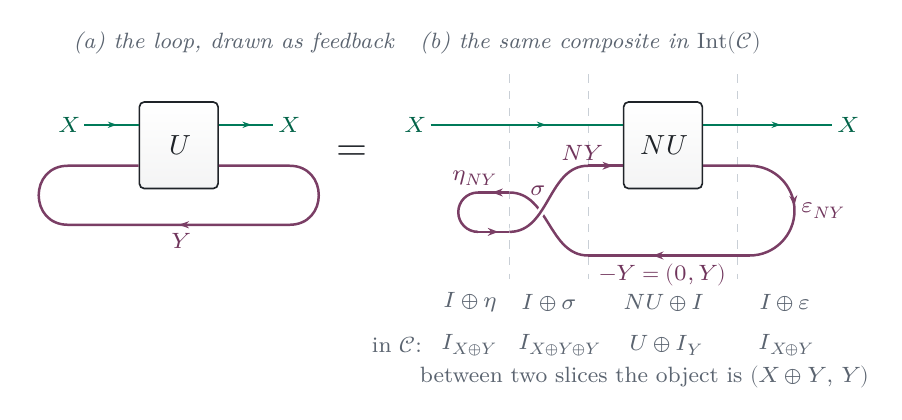
\begin{tikzpicture}[house, x=1mm, y=1mm,
  slice/.style={draw=hairline, dashed, line width=0.45pt},
  cupcap/.style={wback},
  back/.style={wback, postaction={decorate}, decoration={markings, mark=at position .5 with {\arrowreversed{Stealth[length=1.3mm,width=.9mm]}}}}]
\node[panel, anchor=west] at (-6,13) {(a) the loop, drawn as feedback};
\node[body] (U) at (8,0) {$U$};
\draw[wpass,flowmark] (-4,2.6) node[labpass, left] {$X$} -- (U.west |- 0,2.6);
\draw[wpass,flowmark] (U.east |- 0,2.6) -- (20,2.6) node[labpass, right] {$X$};
\feedbackcurve{U}{7.5}{9.5}
\node[labback, anchor=north] at (8,-10.6) {$Y$};
\node[font=\Large] at (30,-1) {$=$};
\begin{scope}[xshift=40mm]
\node[panel, anchor=west] at (-2,13) {(b) the same composite in $\mathrm{Int}(\mathcal C)$};
\foreach \x in {10,20,39} \draw[slice] (\x,9) -- (\x,-17);
\node[lab, text=muted] at (5,-20) {$I\oplus\eta$};
\node[lab, text=muted] at (15,-20) {$I\oplus\sigma$};
\node[lab, text=muted] at (29.5,-20) {$NU\oplus I$};
\node[lab, text=muted] at (45,-20) {$I\oplus\varepsilon$};
\node[lab, text=muted, anchor=east] at (-.5,-25.4) {in $\mathcal C$:};
\node[lab, text=muted] at (4.7,-25.4) {$I_{X\oplus Y}$};
\node[lab, text=muted] at (16.2,-25.4) {$I_{X\oplus Y\oplus Y}$};
\node[lab, text=muted] at (29.7,-25.4) {$U\oplus I_Y$};
\node[lab, text=muted] at (45,-25.4) {$I_{X\oplus Y}$};
\node[note, anchor=north west] at (-2,-27.4) {between two slices the object is $(X\oplus Y,\,Y)$};
\node[body] (V) at (29.5,0) {$NU$};
\draw[wpass,flowmark] (0,2.6) node[labpass, left] {$X$} -- (V.west |- 0,2.6);
\draw[wpass,flowmark] (V.east |- 0,2.6) -- (51,2.6) node[labpass, right] {$X$};
\tikzset{along/.style={postaction={decorate},decoration={markings,
  mark=at position #1 with {\arrow{Stealth[length=1.35mm,width=1mm]}}}}}
\draw[wback,along=.6] (V.east |- 0,-2.6) -- (40.5,-2.6)
  arc[start angle=90,end angle=-90,radius=5.7mm];
\draw[wback,along=.6] (40.5,-14) -- (20,-14);
\draw[wback] (20,-14) to[out=180,in=0] (10,-6);
\draw[wback,along=.55] (10,-6) -- (6,-6);
\draw[wback] (6,-6) arc[start angle=90,end angle=270,radius=2.5mm];
\draw[wback,along=.65] (6,-11) -- (10,-11);
\draw[wback,preaction={draw=white,line width=2.8pt}]
  (10,-11) to[out=0,in=180] (20,-2.6);
\draw[wback,along=.72] (20,-2.6) -- (V.west |- 0,-2.6);
\node[lab, text=backdeep, anchor=south] at (5.4,-5.8) {$\eta_{NY}$};
\node[lab, text=backdeep, anchor=west] at (46.4,-8.3) {$\varepsilon_{NY}$};
\node[labback, anchor=south] at (19,-2.6) {$NY$};
\node[labback, anchor=south] at (13.6,-7.05) {$\sigma$};
\node[labback, anchor=north] at (29.5,-14.4) {$-Y=(0,Y)$};
\end{scope}
\end{tikzpicture}
\end{document}
